
\usetikzlibrary{shapes,arrows}

\newcommand{\hoo}[0]{H_2O}

\tikzstyle{decision} = [diamond, draw, fill=blue!30, text badly centered, node distance=3.5cm, inner sep=3pt]
    
    %  text width=15em
\tikzstyle{block} = [inner sep = 10,rectangle, draw, fill=black!10, text centered, rounded corners, minimum height=5em,node distance=2.5cm]
    
\tikzstyle{line} = [draw, -latex']

\tikzstyle{cloud} = [draw, rectangle,fill=orange!30, node distance=5.5cm,
    minimum height=2em]

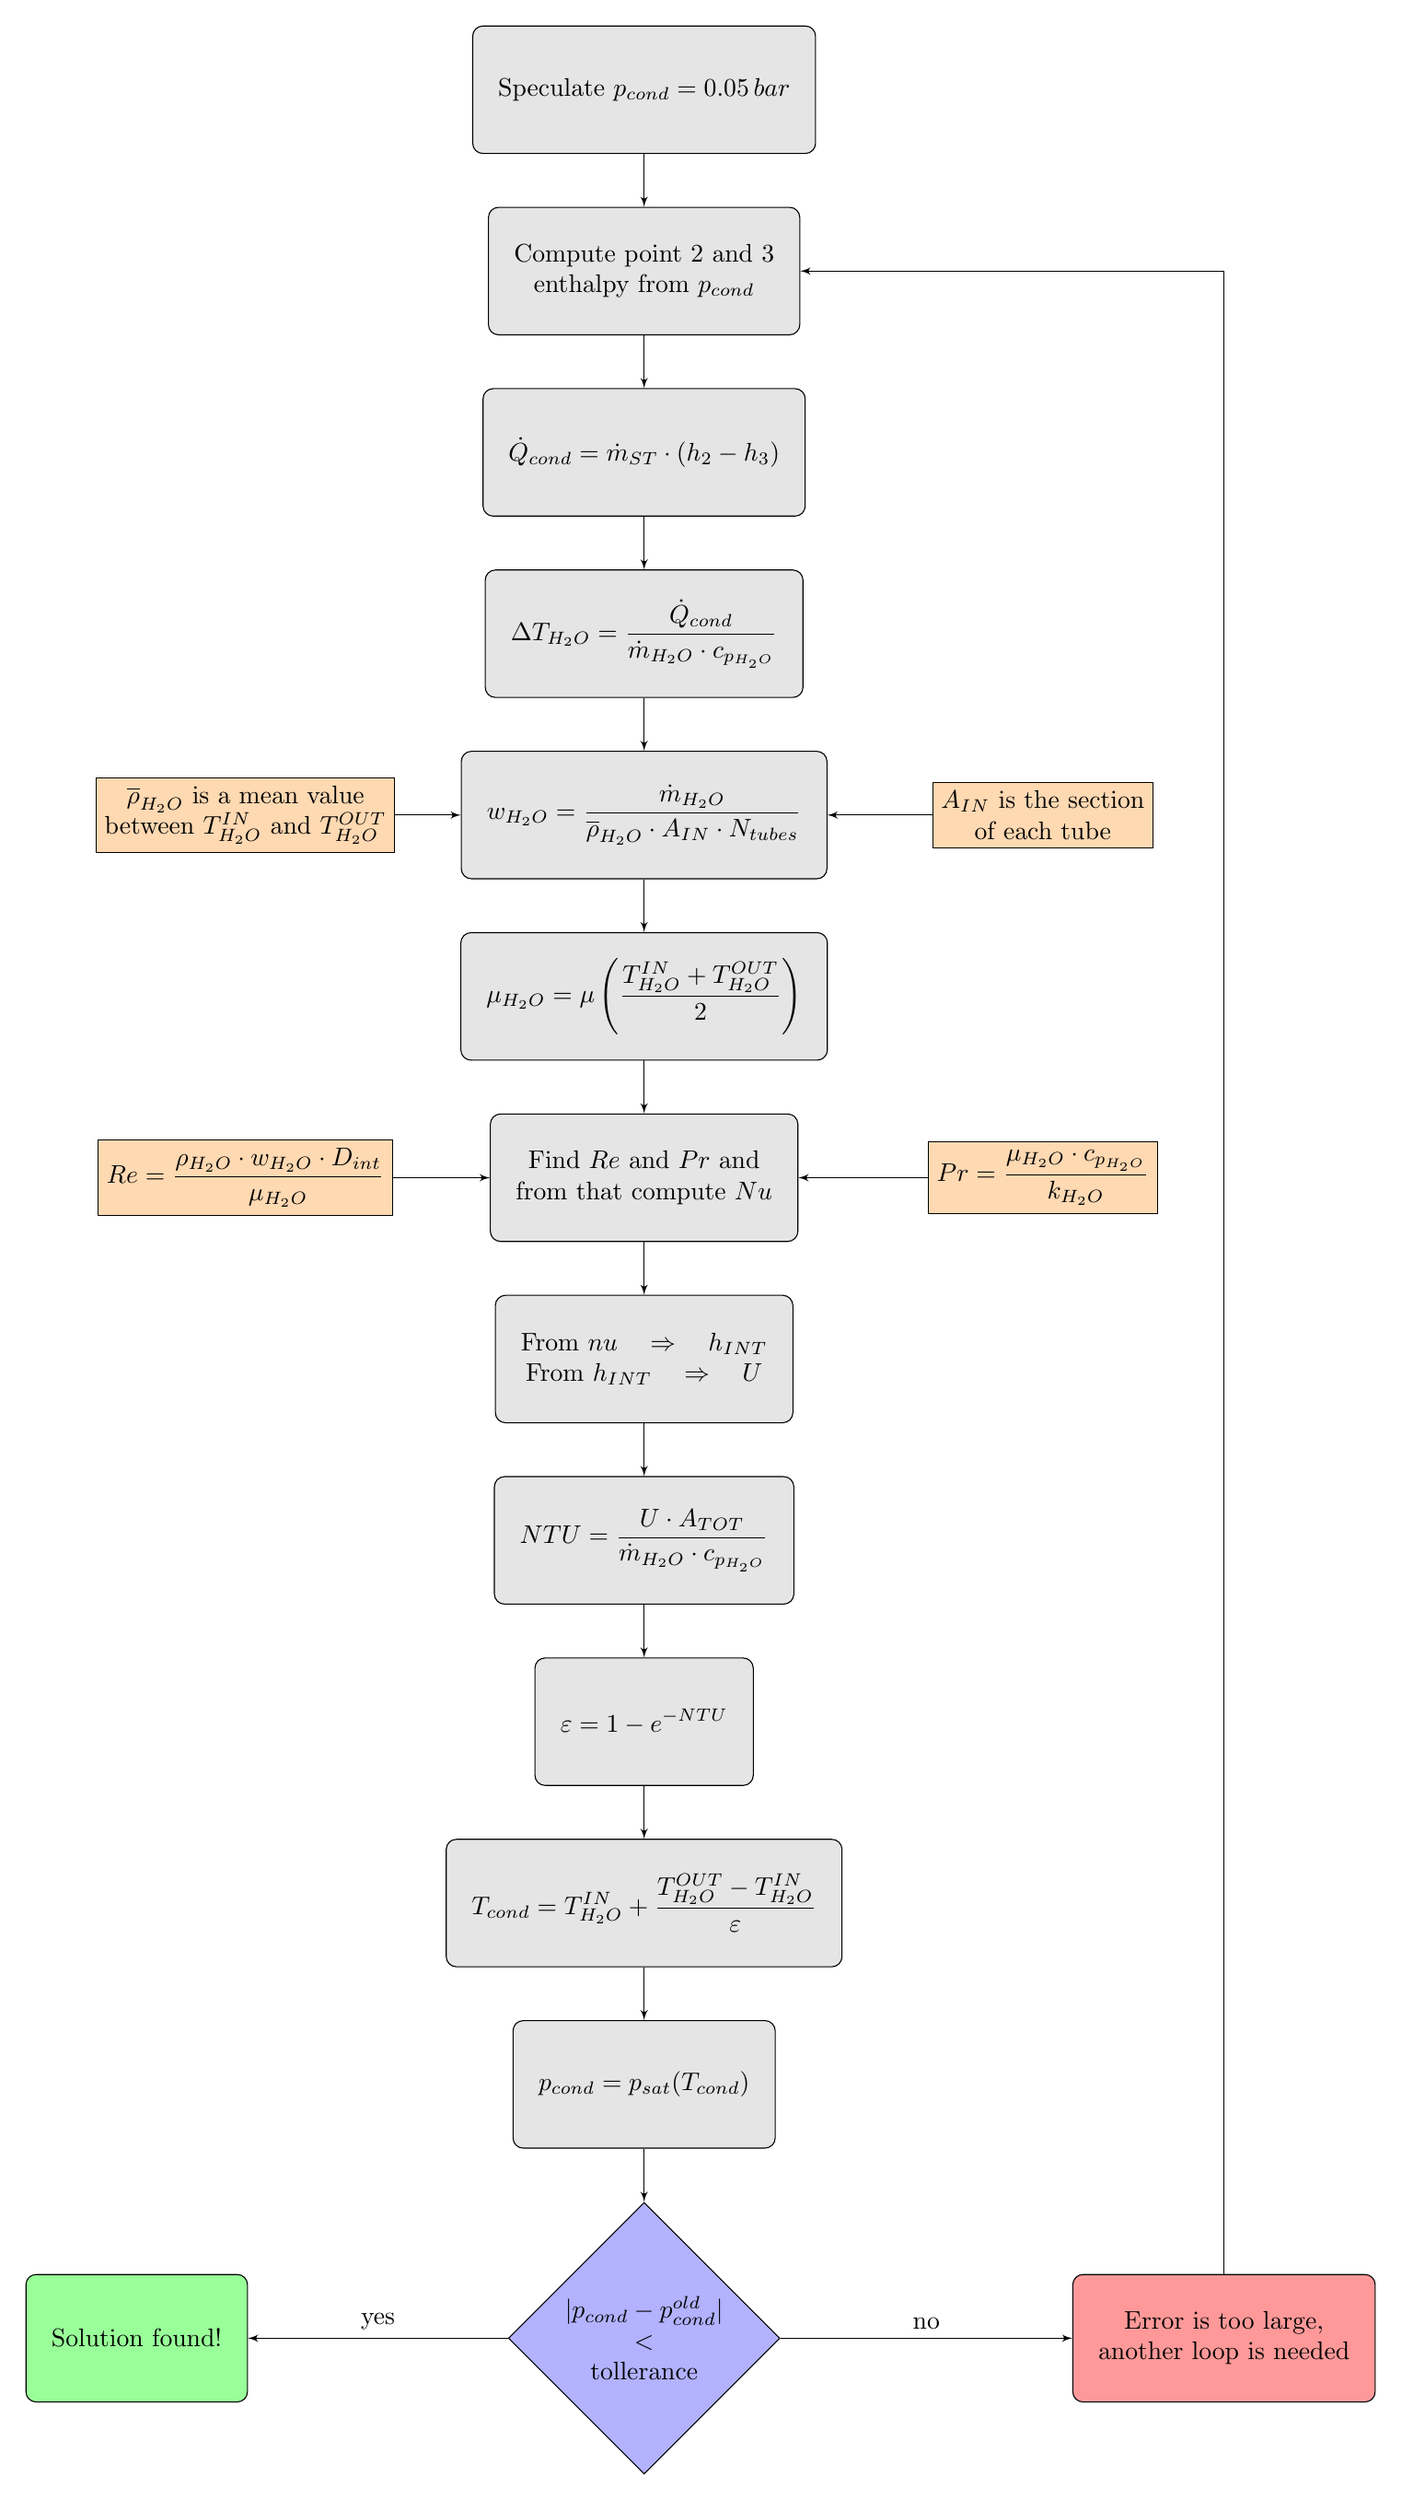
\begin{tikzpicture}
%[node distance = 1cm, auto]


\node [block] (pcond) {Speculate $p_{cond} = 0.05\, bar$};
\node [block, below of=pcond,align=center] (eval_turbine) {Compute point 2 and 3\\ enthalpy from $p_{cond} $};

\node [right of=eval_turbine,node distance=8cm] (null1) {};

\node [block, below of=eval_turbine] (qdot_cond) {$\dot{Q}_{cond} = \dot{m}_{ST} \cdot (h_2-h_3)$};
\node [block, below of=qdot_cond] (Tout) {$\displaystyle \Delta T_{H_2O}= \frac{ \dot{Q}_{cond} }{ \dot{m}_{H_2O} \cdot c_{p_{H_2O}} }$ };
\node [block, below of=Tout] (w_water) {$\displaystyle  w_{H_2O}= \frac{ \dot{m}_{H_2O}  }{ \overline{\rho}_{H_2O} \cdot A_{IN} \cdot N_{tubes} }$ };

%suggestion
\node [cloud, left of=w_water,align=center] (rho_water) {$\overline{\rho}_{H_2O}$ is a mean value\\ between $T_{H_2O}^{IN}$ and $T_{H_2O}^{OUT}$};
\node [cloud, right of=w_water,align=center] (Ain) {$A_{IN}$ is the section \\ of each tube};

\node [block, below of=w_water] (mu) {$\displaystyle \mu_{H_2O} = \mu \left( \frac{ T_{H_2O}^{IN} + T_{H_2O}^{OUT} }{ 2 } \right)$ };
\node [block, below of=mu,align=center] (nu) {Find $Re$ and $Pr$ and \\ from that compute $Nu$ };

%suggestion
\node [cloud, left of=nu,align=center] (re) {$\displaystyle Re = \frac{\rho_{\hoo} \cdot w_{\hoo} \cdot D_{int}}{\mu_{\hoo}}$};
\node [cloud, right of=nu,align=center] (pr) {$\displaystyle Pr = \frac{\mu_{\hoo} \cdot c_{p_{\hoo}}}{k_{\hoo}}$};

\node [block, below of=nu,align=center] (U) {From $nu \quad \Rightarrow  \quad h_{INT}$ \\ From $ h_{INT}  \quad \Rightarrow  \quad U$ };
\node [block, below of=U,align=center] (NTU) {$\displaystyle NTU = \frac{ U\cdot A_{TOT} }{ \dot{m}_{H_2O} \cdot c_{p_{H_2O}} }$};
\node [block, below of=NTU,align=center] (eps) {$\displaystyle \varepsilon = 1- e^{-NTU} $};
\node [block, below of=eps,align=center] (tcond) {$\displaystyle T_{cond} = T_{H_2O}^{IN} + \frac{ T_{H_2O}^{OUT} - T_{H_2O}^{IN} }{ \varepsilon  }$};
\node [block, below of=tcond,align=center] (pcond_new) {$\displaystyle p_{cond} = p_{sat}(T_{cond})$};

\node [decision, below of=pcond_new,align=center] (decide) {$| p_{cond} - p_{cond}^{old} | $\\ $<$ \\tollerance};
    
\node [block,node distance=7cm,fill=green!40, left of=decide,align=center] (yes) {Solution found!};
\node [block,node distance=8cm,fill=red!40, right of=decide,align=center] (no) {Error is too large,\\ another loop is needed};

% arrows
\path [line] (pcond) -- (eval_turbine);
\path [line] (eval_turbine) -- (qdot_cond);
\path [line] (qdot_cond) -- (Tout);
\path [line] (Tout) -- (w_water);

\path [line] (rho_water) -- (w_water) ;
\path [line] (Ain) -- (w_water) ;

\path [line] (w_water) -- (mu);
\path [line] (mu) -- (nu);

\path [line] (re) -- (nu) ;
\path [line] (pr) -- (nu) ;

\path [line] (nu) -- (U);
\path [line] (U) -- (NTU);
\path [line] (NTU) -- (eps);
\path [line] (eps) -- (tcond);
\path [line] (tcond) -- (pcond_new);
\path [line] (pcond_new) -- (decide);

\path [line] (decide) -- node[anchor=south] {yes} (yes);

\path [line] (decide) -- node[anchor=south] {no} (no);

\path [line] (no) |- (eval_turbine) ;
%\path [line] (decide) -| node[near start,anchor=south] {no} (null1) -- (eval_turbine) ;
%\path [line] (-3,0) --++(pcond_new) -| (eval_turbine);

\end{tikzpicture}